\chapter*{Conclusions}
\chaptermark{}

Figure~\ref{fig:phisDGsNew} shows the current status of $\phis$ and $\DGs$ measurements. It is an update of Figure~\ref{fig:phisDGs} in
Section~\ref{subsec:intro_Jpsiphi_decay}, which gives an overview of the status in the Spring of 2014, when only results with the 2011
dataset from LHCb were available. Results of the measurement presented in this thesis, which uses both the 2011 and 2012 LHCb datasets and
was published in \cite{LHCb-PAPER-2014-059}, are shown in combination with the results from measurements in the
\BstoJpsipipi~\cite{LHCb-PAPER-2014-019} and \BstoDspDsm~\cite{LHCb-PAPER-2014-051} decay channels. The other results in the figure are
from a new CMS measurement~\cite{CMS:2014jxa}, the updated \atlas{} measurement~\cite{Aad:2014cqa}, and the CDF~\cite{Aaltonen:2012ie} and
D0~\cite{Abazov:2011ry} measurements in the \BstoJpsiphi{} channel.
\begin{figure}[htb]
  \centering
  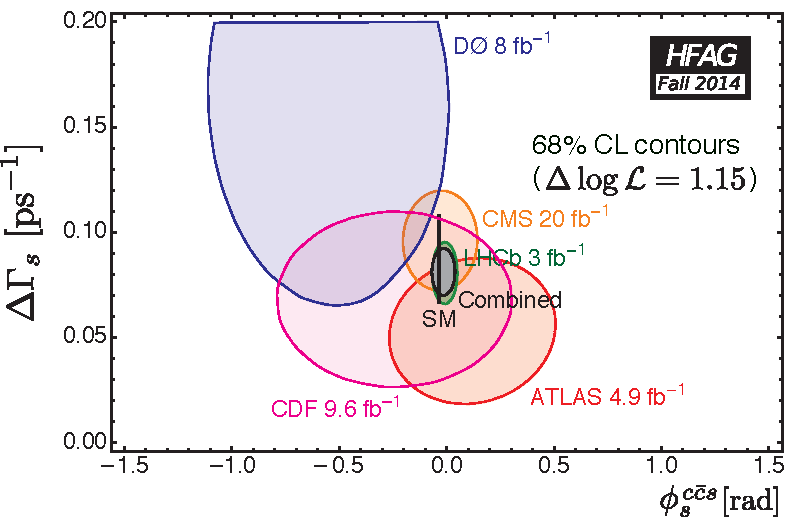
\includegraphics[width=\textwidth]{graphics/results/hfag_Fall2014_DGsphis-cmyk}
  \caption{Combination of $\phis$ (here represented as $\phisccs$) and $\DGs$ measurements by HFAG~\cite{Amhis:2012bh}.
           The estimates at 68\% confidence level (CL) by the different experiments are shown by the coloured contours.
           Note that the LHCb contour (green) is a combination of measurements in the
           \BstoJpsiphi{}, \BstoJpsipipi{}, and \BstoDspDsm{} decays.
           The combined 68\% confidence region is shown by the grey area and the Standard Model prediction by the vertical bar.}
  \label{fig:phisDGsNew}
\end{figure}

The objective of these measurements, as described in Sections~\ref{sec:intro_SM}--\ref{sec:intro_Jpsiphi}, is to test the Standard Model by
comparing the CP violation that is measured in $\btoccs$ transitions to the prediction obtained by interpreting other measurements within
the Standard Model framework. The current combined precision of the $\phis$ result is 0.04\unitsp{}rad, which is equal to the deviation of
the Standard Model prediction from zero. This precision is not yet sufficient to measure potential small deviations from the Standard
Model, but these measurements do rule out large contributions from non-Standard Model physics. As discussed in
Section~\ref{subsec:intro_Jpsiphi_decay}, both experimental and theoretical improvements are required for a more precise analysis of CP
violation in $\btoccs$ transitions.

At lowest order, the decays that are included in the combination of Figure~\ref{fig:phisDGsNew} are governed by a single tree-level
$\btoccs$ transition and CP violation is described by common $\phis$ and $\lamsAbs$ parameters. To compare a more precise measurement of CP
violation to its prediction in the Standard Model, higher order contributions must be considered. These potentially yield CP violation
parameters with different values for each decay and each angular-momentum state contributing to the \BstoJpsiKK{} decay.

Theory: \cite{Liu:2013nea} or \cite{Faller:2008gt}.
